\chapter{Backgrounds}
\label{sec:Backgrounds}

The big disadvantage of semileptonic decays is that the neutrino can't be reconstructed.
At hadron colliders like the \lhc is it impossible to know the initial state, so one doesn't have enough constraints to reconstruct the full kinematic information about the decaying particle.
Being aware of these problems due to experimental setup it is clear that one can't use a well reconstructed \Lb mass peak to separate signal from background.
A main source of background is expected to be the decay \decay{\Bd/\Bp}{\Dz\mun\neumb X} where one randomly combines a proton to this decay.
Ths background is handled by the fit of the \logIP distribution.
Other sources of backgrounds and their possible impact on the obtained signal yield \NDp are discussed in the following.
For the \LbToLcmunu channel it is assumed, that all non-negligible backgrounds are accounted for due to the sidebandsubtraction and including wrong sign events as well as resonant modes components in the fit.
The discussion in this chapter thus refers completely to the \LbToDpmunuX channel.

% ====================================
% section: proton misidentification
% ====================================
\section{Proton misidentification}
A possible source of backgrounds is that one misinterprets a decay as \LbToDpmunuX since one misidentifies a final state particle.
In this analysis it is most likely that the proton is misidentified since the final state pion and kaon are reconstructed to a \Dz yielding in a nice peak and the muon leaves a clear signature in the detector due to its relatively long lifetime and low interaction with matter.
Examples for these kind of backgrounds are the decays \decay{\Bs}{\Dz\Kp\mun\neumb X} and \decay{\Bd/\Bp}{\Dz\pip\mun\neumb X}, where either the \Kp or \pip is misidentified as proton.
Though there are tight requirements on the proton identification at selection stage, the data will still be polluted by misidentified particles.
To identify the amount of misidentified protons, a slightly different data sample than the nominal one is used. 
In this sample no requirements on the proton idenfication are applied.
Except for those all other requirements are the same as described in section \ref{sec:Selection}.
However the removal of the particle identification requirements lets the data size of the sample rapidly increase.
To keep the data size acceptable a so called 5\% prescaling has been applied, i.e. only 5\% of all events are actually stored.
The decision if a particle is stored or not is made by random.
That's why absolute numbers quoted in this section can't be compared to the obtained signal yields etc. in the previous sections.
The study on misidentified backgrounds is done in three steps.

\subsection{Definition of particle identification regions - Number of particle candidates}
\label{sec:PIDCalib_Ncand}
As a first step it has to be defined what requirements have to e fulfilled, that a particle is called a proton, pion or kaon.
Therefore the PID (for Particle IDentification) variables are used.
Remember, that \lhcb's particle idenitfication system provides likelihoods for each particle hypothesis.
The PID variables now describe differences between the logarithms of these likelihoods, e.g. PIDp is defined as the difference of the logarithmic likelhoods between the proton and pion hypothesis.
A value of PIDp$>0$ hence means, that the particle is more likely a proton than a pion.
Respectively, the PIDK compares kaon to pion hypothesis.
If one wants to separate protons from kaons it is useful to look at PIDp$-$PIDK.
The definition what will be called proton is motivated by the requirements applied in the analysis (see section \ref{sec:Selection}). 
In detail the regions for the identification of protons, pions and kaons are:
\begin{itemize}
\item proton: $\text{PIDp} - \text{PIDK} > 10.0 \text{ and } \text{PIDp} > 10.0$
\item pion: $\text{PIDp} < 10.0 \text{ and } \text{PIDK} < 0.0$
\item kaon: $\text{PIDp} - \text{PIDK} < 10.0 \text{ and } \text{PIDK} > 0.0$
\end{itemize}

Furthermore these regions and their population are visualised in figure \ref{fig:PIDregions}. 
From this the number of candidates for each particle species is obtained, in the following denoted as \Ncand{i}, with $i \in \left[\pi, \kaon, \proton\right]$. 
The number of candidates are
\begin{align}
    \Ncand{\pi}     &= \PIDNcandpionval \pm \PIDNcandpionerr, \\ 
    \Ncand{\kaon}   &= \PIDNcandkaonval \pm \PIDNcandkaonerr, \\ 
    \Ncand{\proton} &= \PIDNcandprotonval \pm \PIDNcandprotonerr.
\end{align}
\begin{figure}[hptb]
	\centering
	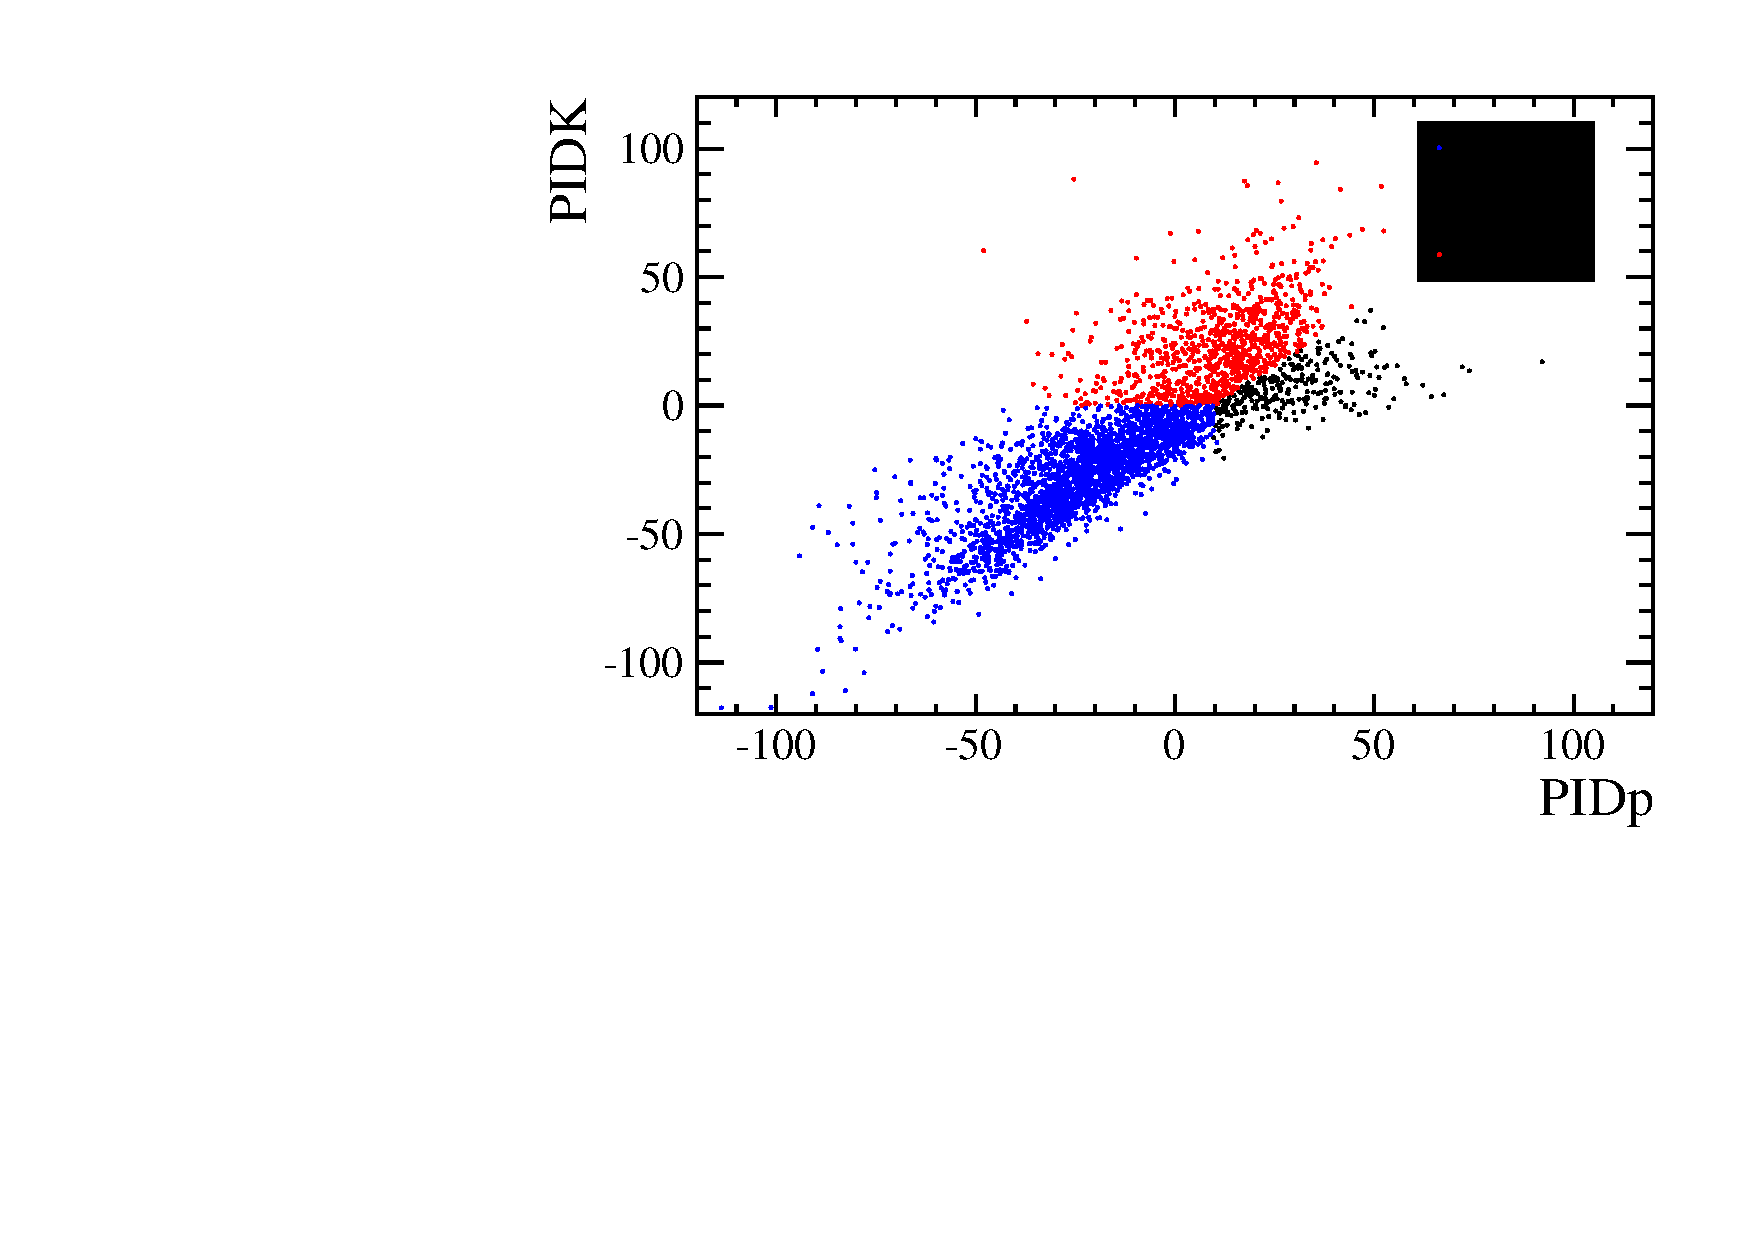
\includegraphics[width=0.49\textwidth]{LbToD0p/PID/PIDK_vs_PIDp}
	\caption{Defined regions for the number of particle candidates.}
	\label{fig:PIDregions}
\end{figure}


\subsection{Determination of ``true" candidates with PID efficiencies}
Of course, this choice of regions is a bit arbitrary and it doesn't prevent real protons, pions and kaons to enter the other regions.
With the PID variables it is only possible to increase or decrease the probability, that a particle enters a ``foreign" region.
Thus, one needs to determine the efficiencies that a real proton, pion or kaon passes the requirements for the identification of being a proton, kaon or pion.
For this purpose the \lhcb PIDcalib tool is used.
This tool includes calibration samples of decays cleanly reconstructed without use of the PID variables for instance the decay \decay{\Lambda}{\proton\pim} for the proton efficiencies.
Since no requirement on the PID has been applied before, it is now possible to study the impact of these requirements.
The PID efficiency for each of the 9 possible combinations (real particle to be identified as other particle according to PID) is determined binwise depending on the particle momentum. 
The results can be seen in figure \ref{fig:PIDefficiencies}.
\begin{figure}[hptb]
	\centering
	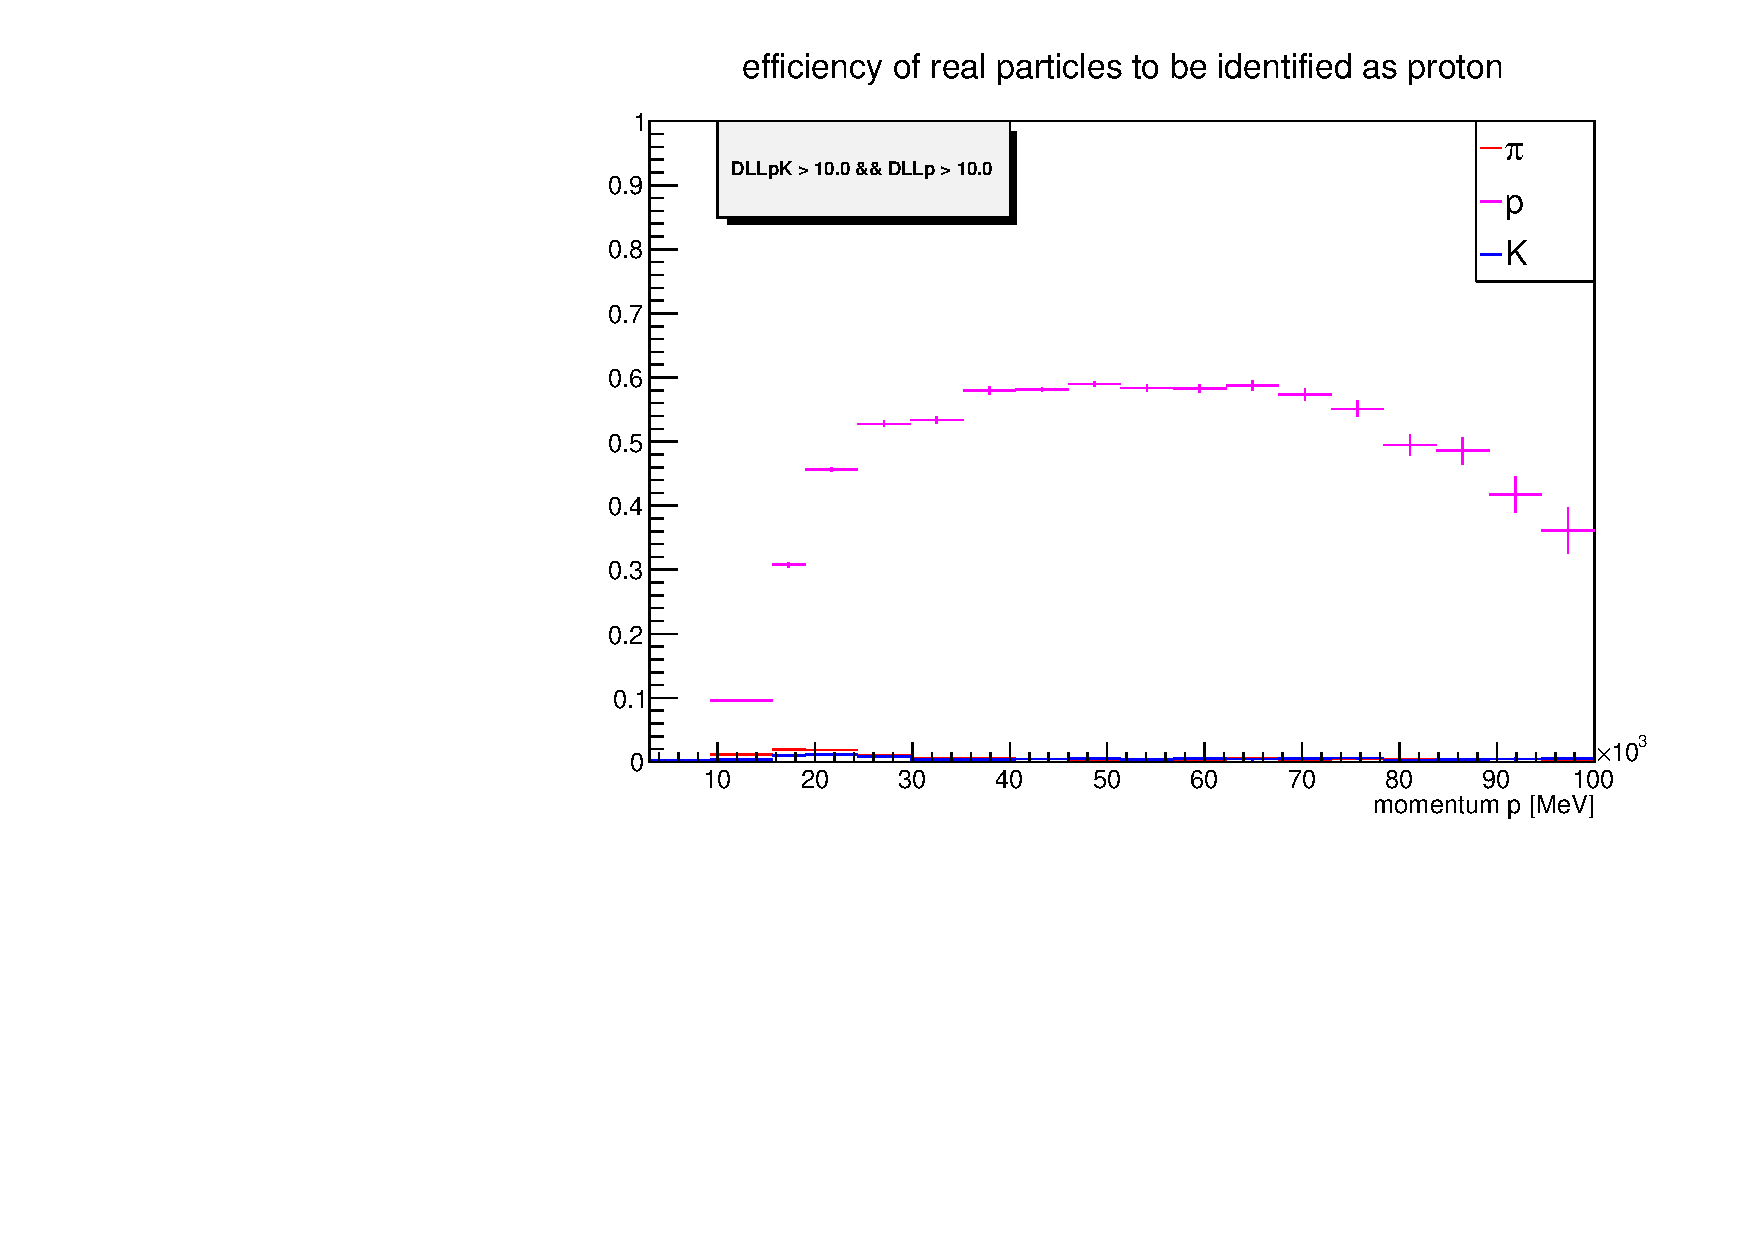
\includegraphics[width=0.32\textwidth]{LbToD0p/PID/PID_proton}
	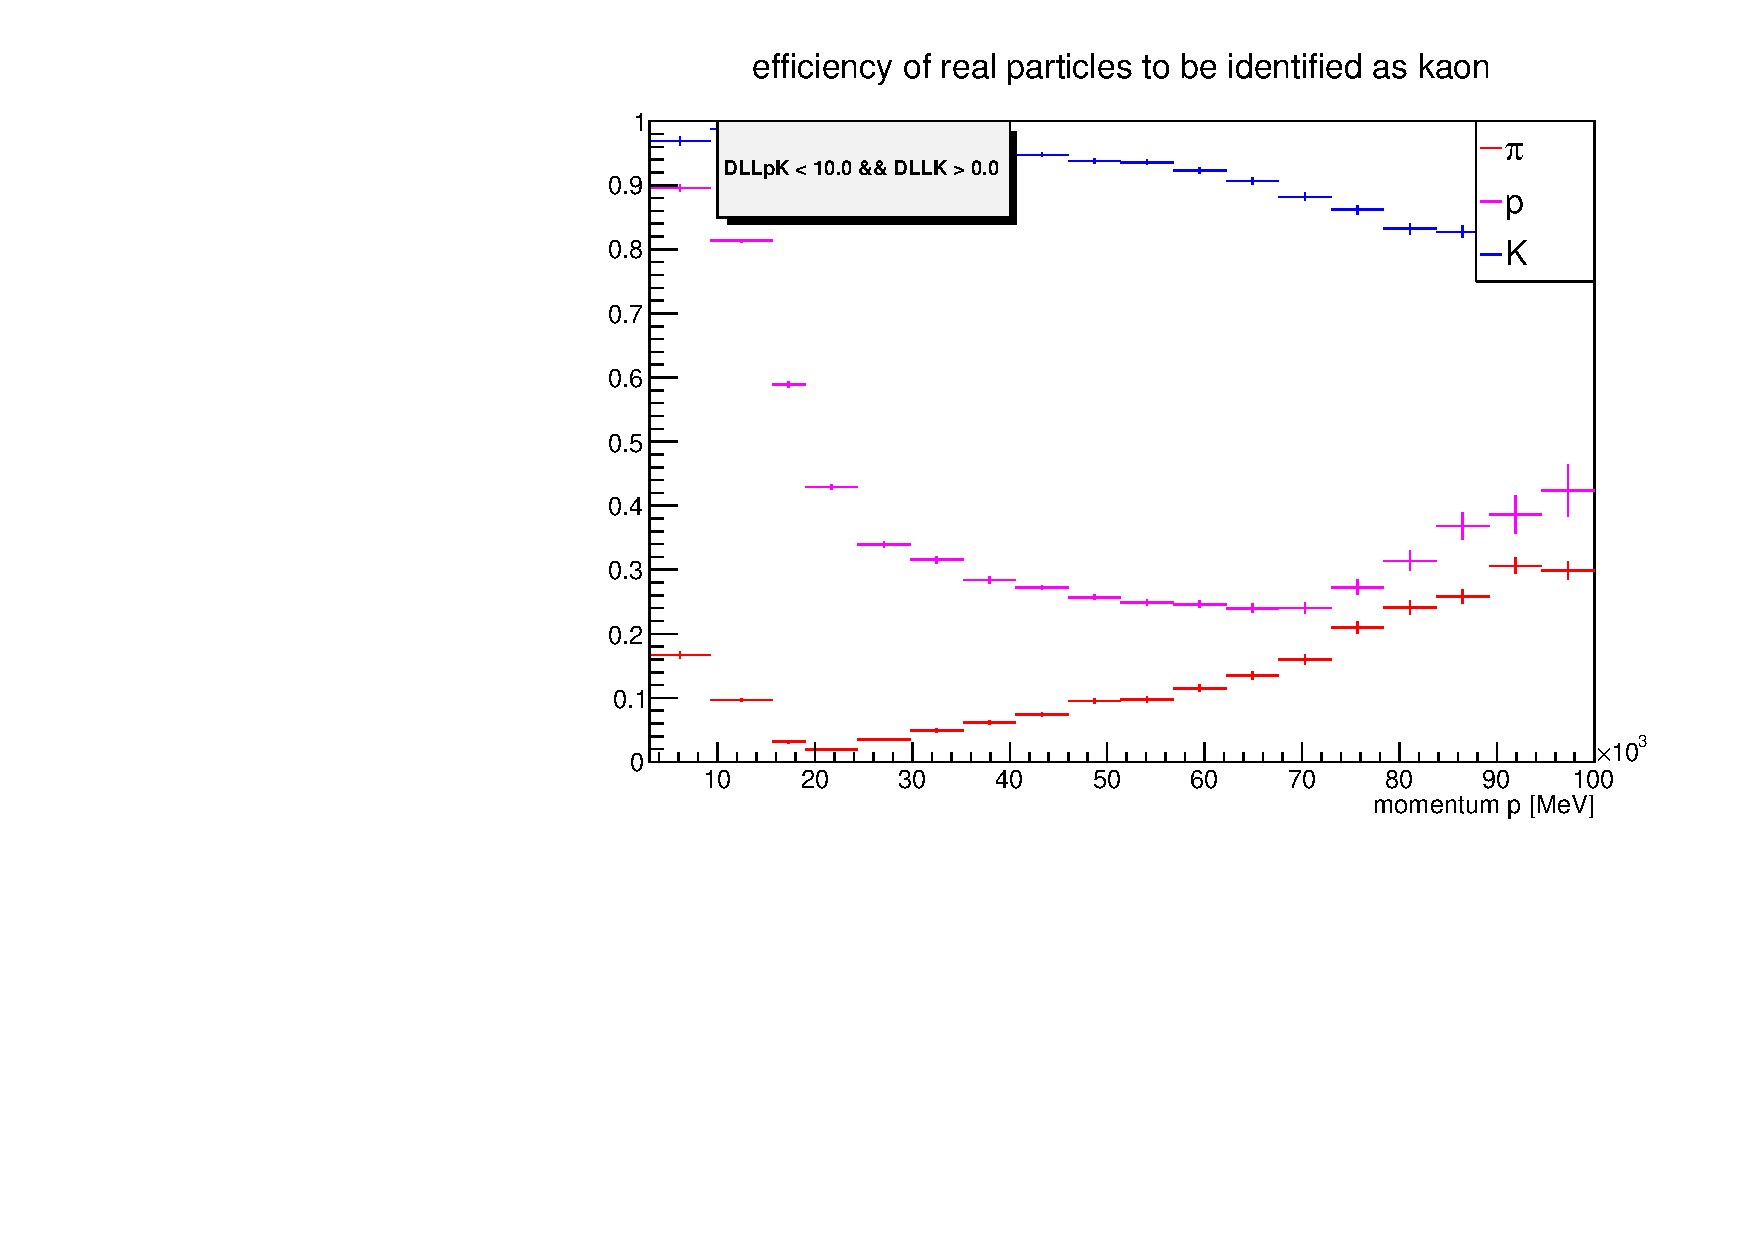
\includegraphics[width=0.32\textwidth]{LbToD0p/PID/PID_kaon}
	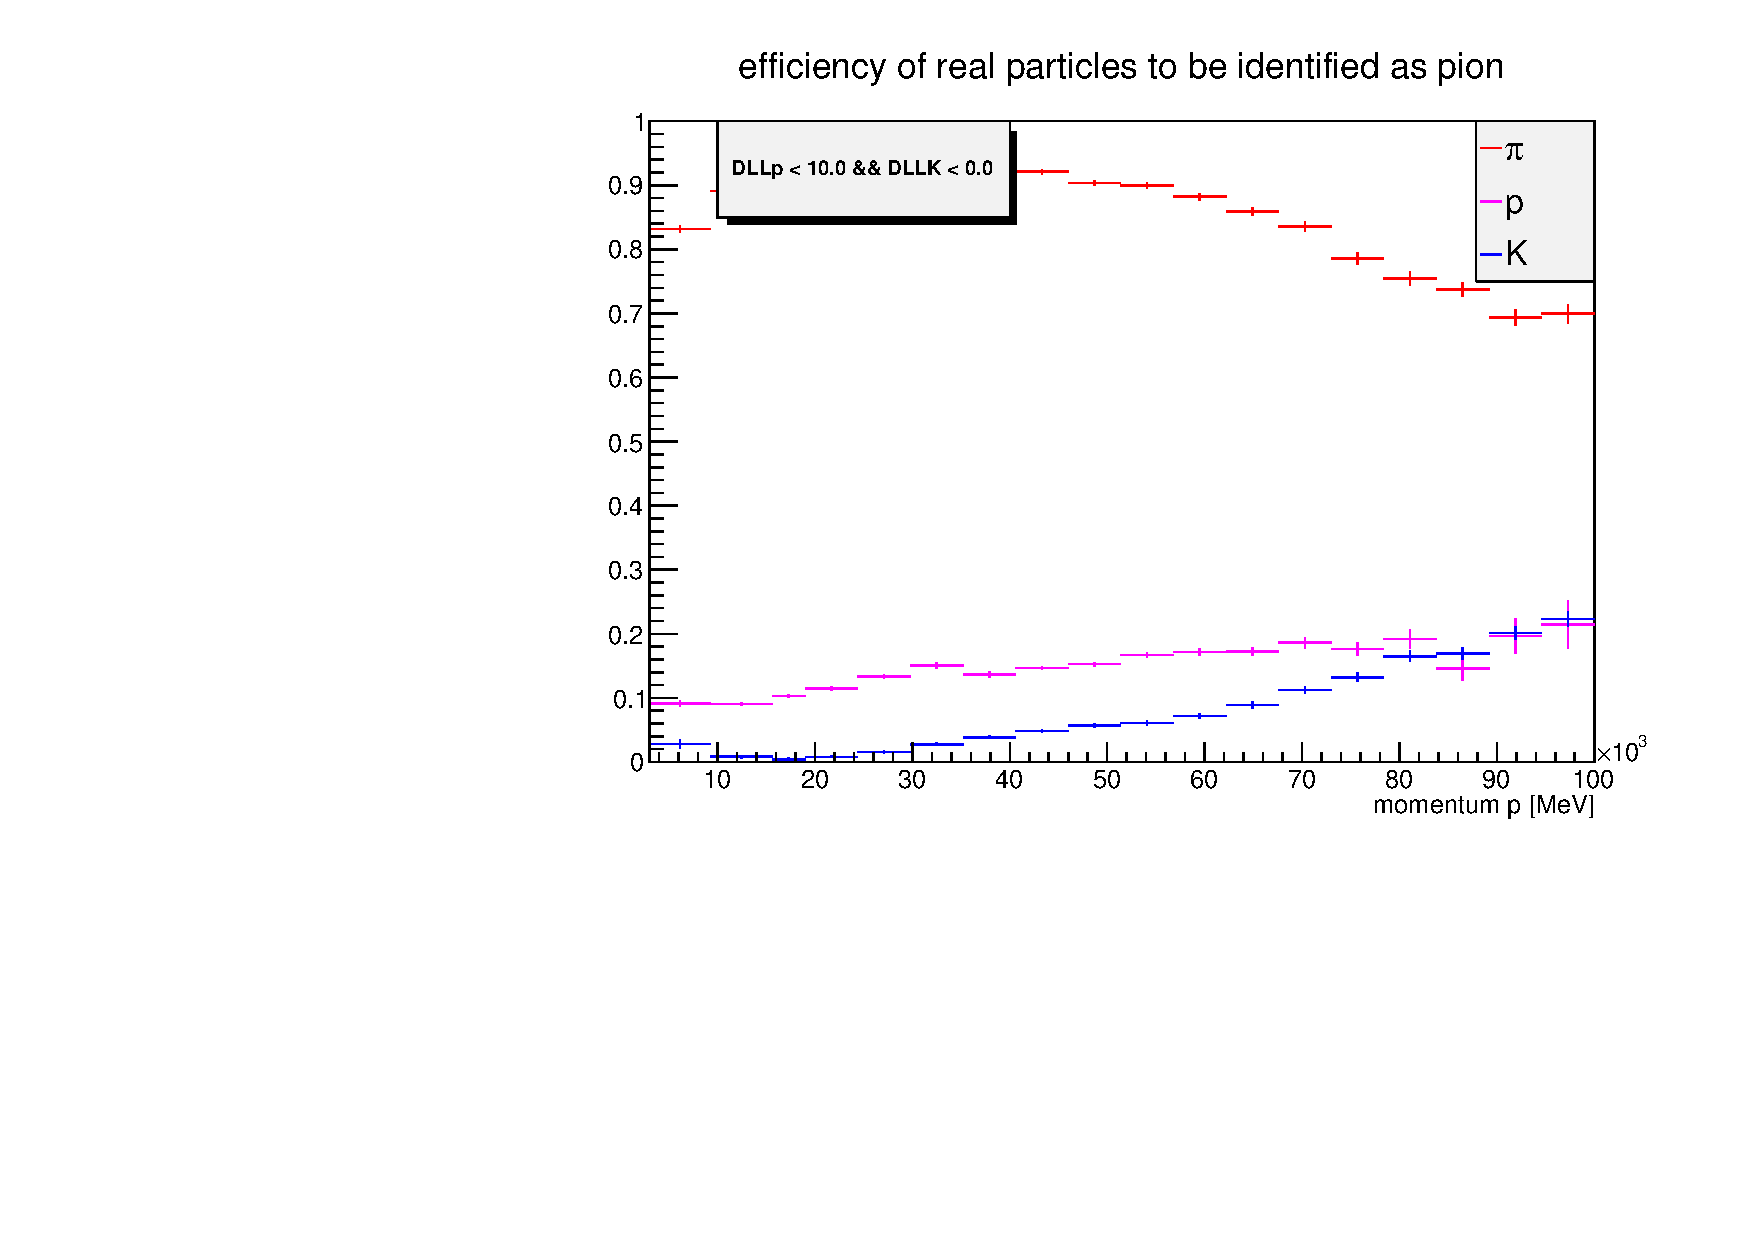
\includegraphics[width=0.32\textwidth]{LbToD0p/PID/PID_pion}
	\caption{Efficiencies that real protons, kaons and pions are identified as protons (left), kaons (middle) or pions (right). The tight requirements on the proton PID applied in this analysis ensures that only few kaons and pions enter the proton region paying the prize, that one looses a lot of
    protons as well.}
	\label{fig:PIDefficiencies}
\end{figure}
To determine a final value for each efficiency, these histograms are weighted with respect to the kinematic distribution of this analysis' data sample. 
The result is:
\begin{align*}        
\begin{pmatrix}
    \effPID{\pip}{\pip}    & \effPID{\Km}{\pip}    & \effPID{\proton}{\pip} \\
    \effPID{\pip}{\Km}     & \effPID{\Km}{\Km}     & \effPID{\proton}{\Km} \\
    \effPID{\pip}{\proton} & \effPID{\Km}{\proton} & \effPID{\proton}{\proton} 
\end{pmatrix}
=
\begin{pmatrix}
0.9409 & 0.0241 & 0.1309 \\
 0.0474 & 0.9681 & 0.3798 \\
 0.0117 & 0.0077 & 0.4893
\end{pmatrix}
\end{align*}

Here, \effPID{i}{j} denotes the efficiency, that a real (true) particle $i$ is identified as what is call $j$ according to the particle regions defined in section \ref{sec:PIDCalib_Ncand}. 
For the following steps, PID efficiency errors are assumed to be negligible compared to the corresponding uncertainties of the particle candidates \Ncand{i}.
With the PID efficiencies \effPID{i}{j} and the number of particle candidates \Ncand{k}, the number of real (true) particles can now be estimated by solving the matrix equation
\begin{align*}
    \begin{pmatrix} 
        \Ncand{\pi} \\ \Ncand{\kaon} \\ \Ncand{\proton}
    \end{pmatrix}
    =
    \begin{pmatrix}
       \effPID{\pi}{\pi}     & \effPID{\kaon}{\pi}     & \effPID{\proton}{\pi} \\
       \effPID{\pi}{\kaon}   & \effPID{\kaon}{\kaon}   & \effPID{\proton}{\kaon} \\
       \effPID{\pi}{\proton} & \effPID{\kaon}{\proton} & \effPID{\proton}{\proton} 
    \end{pmatrix}
    \begin{pmatrix} 
        \Ntrue{\pi} \\ \Ntrue{\kaon} \\ \Ntrue{\proton }
    \end{pmatrix},
\end{align*}
which delivers
\begin{align}
    \Ntrue{\pi}     &= \PIDNtruepionval \pm \PIDNtruepionerr, \\ 
    \Ntrue{\kaon}   &= \PIDNtruekaonval \pm \PIDNtruekaonerr, \\ 
    \Ntrue{\proton} &= \PIDNtrueprotonval \pm \PIDNtrueprotonerr.
\end{align}
\Ntrue{i} denotes the number of real particles $i$ in the sample.

\subsection{Estimate of misidentified protons}
Using the results of the previous subsections it is now possible to estimate the number of misidentified protons, i.e.``true" kaons or pions entering the proton region.
This is calculated by multiplying the number of ``true" particles \Ntrue{i} with the PID efficiency \effPID{i}{\proton} to be identified as proton. 
\begin{align}
    N^{\pi}     &= \effPID{\pi}{\proton} \Ntrue{\pi}         = \PIDNtruePregionpionval \pm \PIDNtruePregionpionerr, \\  
    N^{\kaon}   &= \effPID{\kaon}{\proton} \Ntrue{\kaon}     = \PIDNtruePregionkaonval \pm \PIDNtruePregionkaonerr, \\ 
    N^{\proton} &= \effPID{\proton}{\proton} \Ntrue{\proton} = \PIDNtruePregionprotonval \pm \PIDNtruePregionprotonerr.
\end{align}
Thus, the amount of misidentified protons is at a single-digit percent level, namely $(\misIDratioval \pm \misIDratioerr)\%$. 
Note again, that the absolute values can't be compared to the signal yields obtained in previous parts of this analysis.
It is only the lastly quoted ratio which can be used in the following.

\section{Misidentified muons}
Though not as prominent as misidentified protons, the misidentification of muons is also considered.
One possibility is that the muon is misidentified from an exclusive 3 body decay of the \Lb for instance \decay{\Lb}{\Dz\proton\pim}.
If this is the case, the decay isn't semileptonic but rather hadronic.
Consequently, the \Lb can be fully reconstructed since all final state particles are seen.
This should lead to a peak in the invariant \Dz\proton\mun around the \Lb mass.
There's indeed such a peak as figure \ref{fig:plot_D0pmuMass} shows.
These kind of backgrounds can thus easily eliminated by vetoing \Dz\proton\muon masses around the \Lb mass, in this case all masses above 5500\mev.
\begin{figure}[hptb]
	\centering
	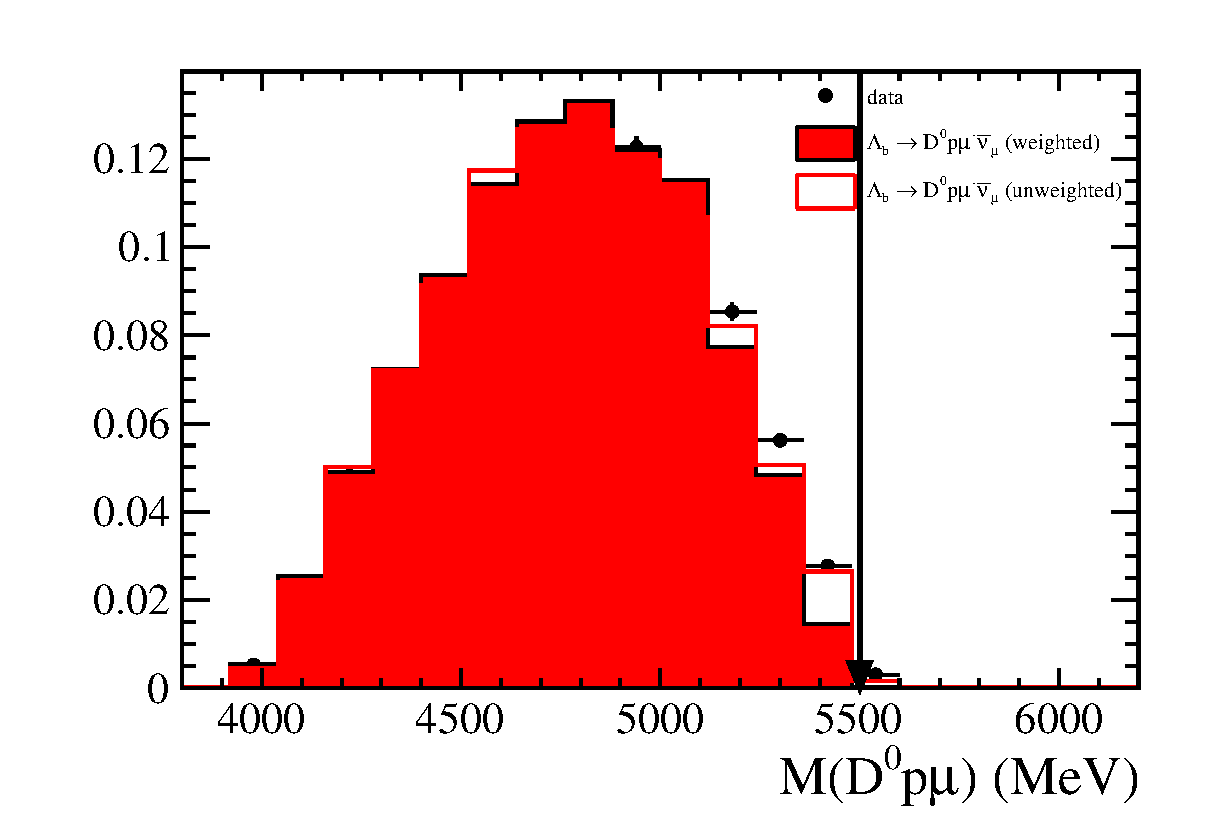
\includegraphics[width=0.49\textwidth]{LbToD0p/plots/data/Bh_M}
	\caption{Invariant \Dz\proton\mun mass. A peak at \Lb mass ($\approx 5620 \mev$) can be seen caused by misidentified muons coming from hadronic decays like \decay{\Lb}{\Dz\proton\pi} where the pion is misidentified as muon. 
             A veto on the \Dz\proton\mun mass indicated by the arrow eliminates such backgrounds.}
	\label{fig:plot_D0pmuMass}
\end{figure}

The situation becomes more tricky, if the background is coming from a more body \Lb decay, i.e. a decay with more than 3 final state particles.
Since this analysis aims to measure the inclusive branching ratio \BR(\LbToDpmunuX), misidentified muons could also come from decays like \decay{\Lb}{\Dz\proton 3\pi}, where one of the 3 pions is misidentified as muon.
These backgrounds aren't easy to eliminate, since the other 2 pions aren't reconstructed and thus not peaking in \Dz\proton\mun mass.
Nonetheless if they're existent in the data sample it might be possible, that such backgrounds tend to sit at lower PIDmu of the muon saying the lower the PIDmu of a muon is the more likely it is to be a misidentified particle.
Unfortunately no distinct structures can be seen in figure \ref{fig:plot_D0pmuMass_vs_muPIDmu}.
This might be a hint that these backgrounds play a minor role.
Assuming that the decay \decay{\Lb}{\Dz\proton 3\pi} behaves in comparison to \decay{\Lb}{\Dz\proton\pim} similar to the Meson decays \decay{\Bd}{\Dm 3\pi} and \decay{\Bd}{\Dm\pip} with 
$\BR(\decay{\Bd}{\Dm 3\pi}) = (2.76 \pm 0.13) \cdot 10^{-3} \approx$ 
$\BR(\decay{\Bd}{\Dm\pip}) = (2.68 \pm 0.13) \cdot 10^{-3}$ (see \cite{PDG})
they should have similar branching ratios and thus should equally leak as background into this analysis.
A comparison with $\BR(\decay{\Bd}{\Dm 3\pi})/\BR(\decay{\Bd}{\Dm\ellp\neul}) \approx 10\%$ and the misidentification probabilty of a hadron of less than $10\%$ \cite{muonID_Performance} justifies the assumption that this background leaks with about $1\%$ in the signal yield.
To account for other possible but not yet measured peaking backgrounds such as \decay{\Lb}{\Dz\proton\rhom}, \decay{\Lb}{\Dz\proton\pim\rhoz} and so on a total peaking background ratio of $(5.0 \pm 2.5)\%$ is assumed.
\begin{figure}[hptb]
	\centering
	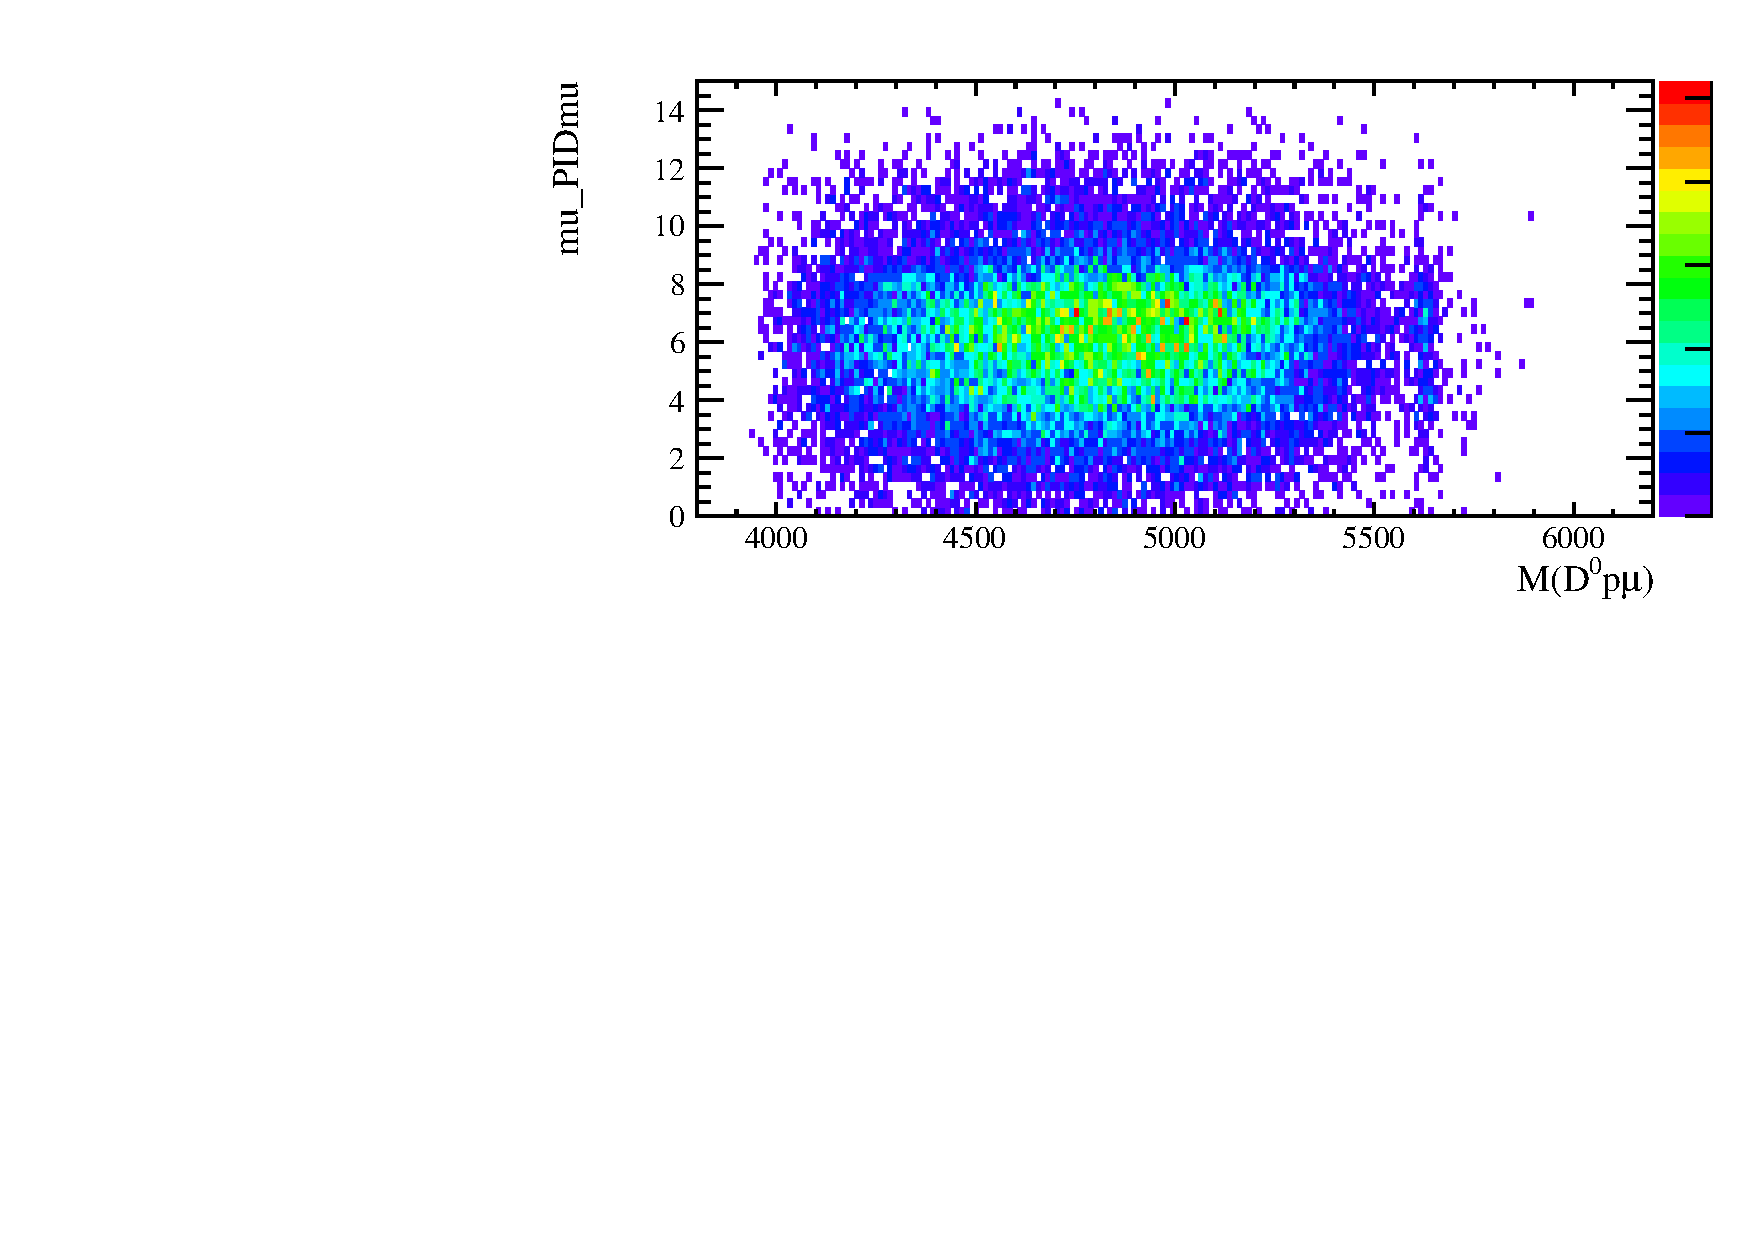
\includegraphics[width=0.49\textwidth]{LbToD0p/plots/data/Bh_M_vs_mu_PIDmu_RS}
	\caption{Invariant \Dz\proton\mun mass versus PIDmu of the muon. No structures tending to low PIDmu can be seen.}
	\label{fig:plot_D0pmuMass_vs_muPIDmu}
\end{figure}

\section{Prompt \Dz}
With prompt \Dz one denotes \Dz coming directly from the primary \proton\proton interaction being not a product of other decaying particles.
The production of prompt charm and hence prompt \Dz is usually a lot higher than the production of \Lb baryons. 
One typically measures a ``few" percent prompt charm background in semileptonic \bquark-hadron decays.
As crosscheck the logarithm of the \Dz impact parameter with respect to the primary vertex is plotted.
Prompt \Dz should have a smaller impact parameter compared to \Dz coming from the \Lb decay.
This should become more clearly visible in wrong sign combinations.
With a view to figure \ref{fig:plot_D0_IP} no discrepancies between data and different wrong sign combinations can bee seen which would indicate the influence of prompt \Dz backgrounds.
Compared to other background sources this kind of background seems to be negligible having furthermore in mind that there are additional cuts applied to combine the \Dz with the other particles to form a \Lb candidate.
\begin{figure}[hptb]
	\centering
	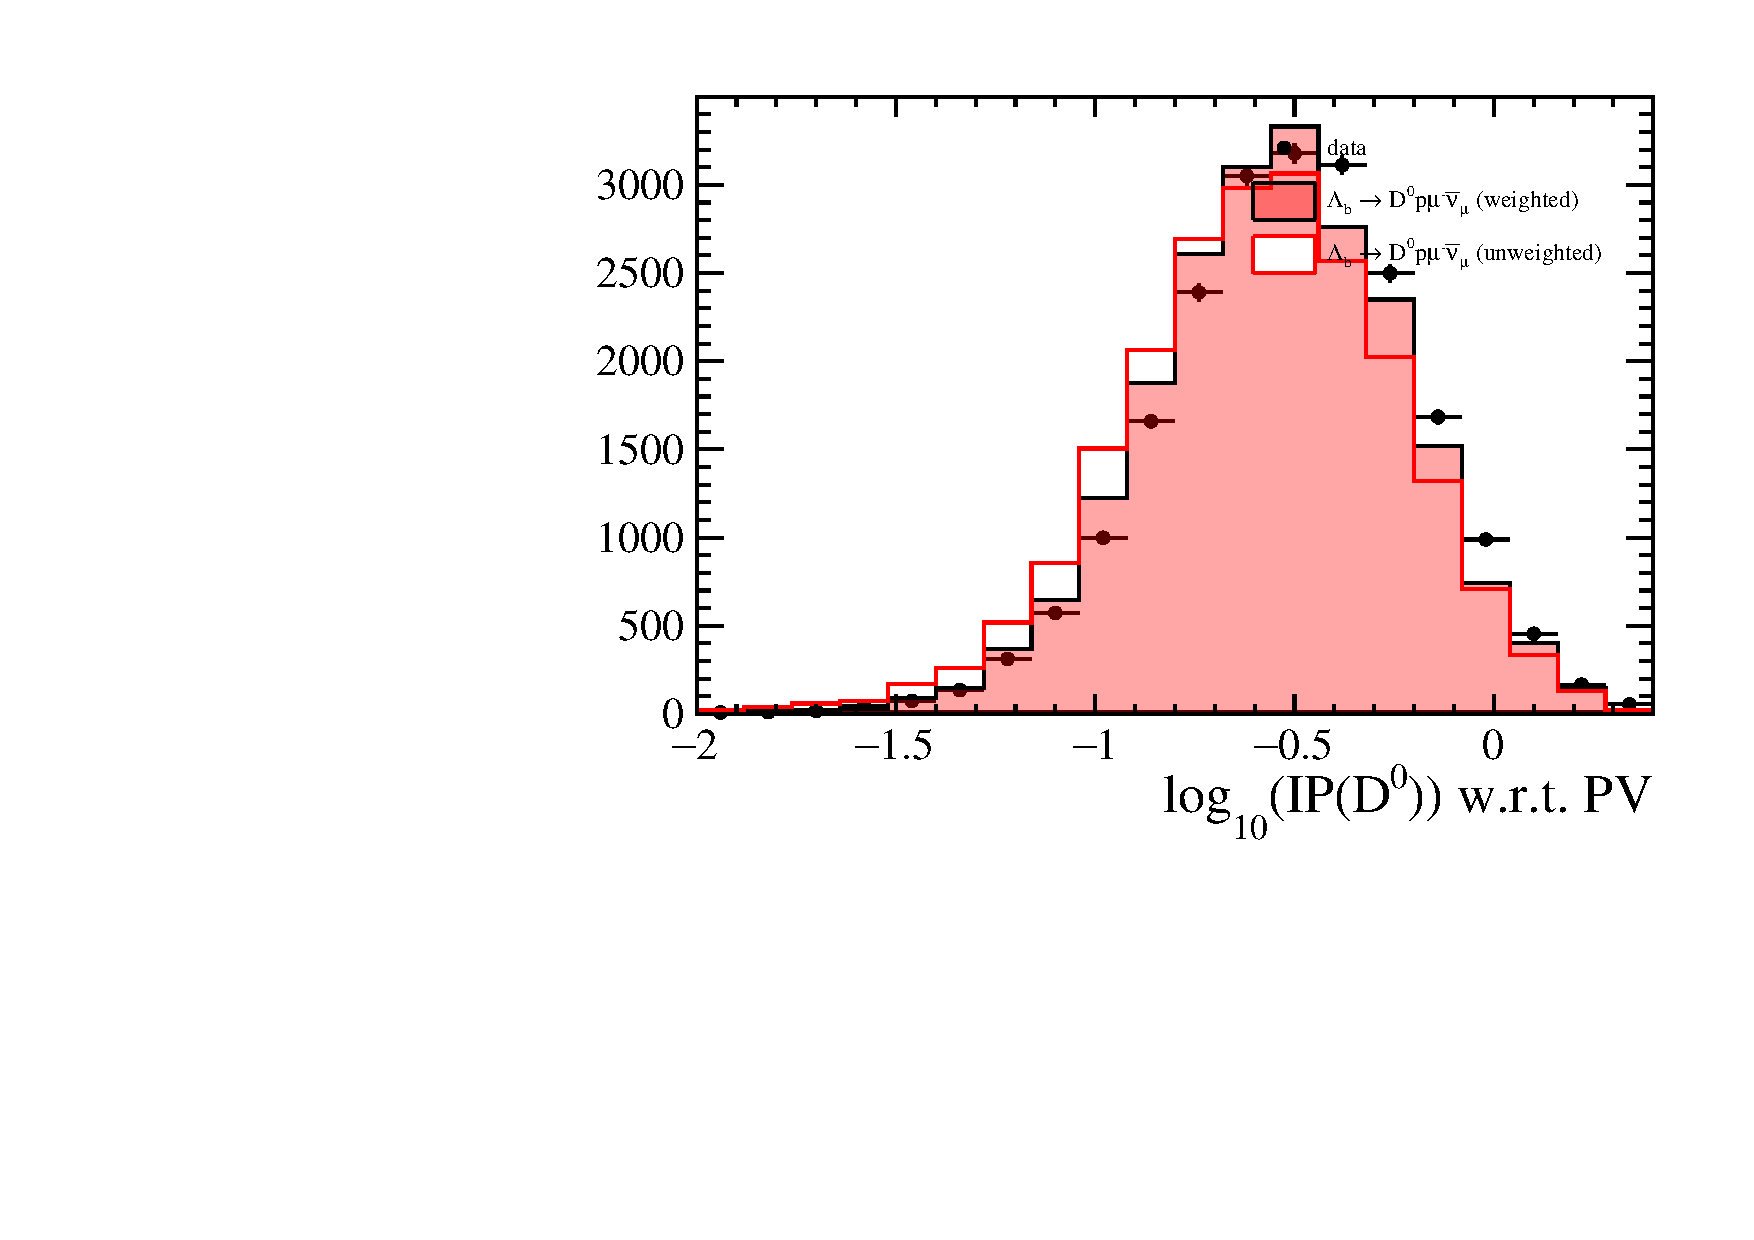
\includegraphics[width=0.49\textwidth]{LbToD0p/plots/data/D0_IP_OWNPV}
	\caption{Logarithm of the \Dz impact parameter with respect to the primary \proton\proton interaction. No special behaviour indicating prompt \Dz background can be seen.}
	\label{fig:plot_D0_IP}
\end{figure}

\section{Other possible backgrounds}
In this section some possible backgrounds not being studied in this analysis are mentioned.
Some of the decays mentioned here haven't been measured or seen so far but should be possible.
\begin{itemize}
    \item $\Lambda_b^0 \rightarrow \Dm \Lc$ \\
          This decay hasn't been measured but it should have a branching ratio of around $10^{-2}$, similar to $B \rightarrow D D_s$.
          If the \Lc decays to \pKpi, there should be another $4 \times 10^{-2}$ and in addition one needs to get the muon from somewhere else, or it has to be from $\Km \rightarrow \mun$ misidentifaction. 
          The vertex quality will be spoilt by the \Lc flight.
          Taking all these arguments together, this should be a sub-percent-level background and thus negligible in this study.
    \item \decay{\Lb}{\Lc N^* \mu \nu} \\
          Here, $N^*$ denotes an excited nucleon states.
          Compared to the previous decay, one can get the muon and proton without any misidentification.
          But this should violate baryon number conservation.
    \item $\Lambda_b^0 \rightarrow D^0 D^- p$ \\
          This decay hasn't been measured but it should be similar to $B \rightarrow DDK$ at a few times $10^{-3}$.
          The inclusive $\Dm \rightarrow \mun X$ branching fraction is about $10^{-2}$.
          So this might be still a percent level background.
    \item prompt \LcResI or \LcResII decays with a \mun from somewhere else \\
          This background should be reduced by requiring the \LcResI resp. \LcResII vertex to be well separated from the PV as done by the combination with a muon to make a \Lb candidate.
    \item \decay{\SigmabRes}{\Lb \pi}, \\ 
          where the pion isn't reconstructed.
          The knowledge about \SigmabRes is very poor.
          The production of \SigmabRes compared to \Lb should be much smaller.
\end{itemize}

\section{Backgrounds summary and estimate of background yield}
The largest background contributions leaking into the signal yield \NDp obtained by the twodimensional fit are discussed to come from either misidentified protons or muons.
All other backgrounds seems to be negligible compared to the latter ones.
Adding them up leads to a total ratio of background events in the signal yield of $(\NDpBKGratioval \pm \NDpBKGratioerr)\%$.
This corresponds to a number of background events of 
\begin{align*}
    \NBgdDp = \NDpBKGval \pm \NDpBKGerr.
\end{align*}
Note that the error on the background ratio goes into the systematic uncertainties.
